\documentclass{article}
\usepackage[utf8]{inputenc}

\usepackage{graphicx}
\usepackage[margin=1.0in]{geometry}

\title{Comparison of Absolute and Relative Pointing Effectiveness using Leap Motion}
\author{ Chris Blythe \and Payel Bandyopadhyay \and Farbod Berenjegani \and Afaque Hussain \and Maninder Singh}
\date{November  2013}

\begin{document}

\maketitle

\section{Abstract}
This project shows an application that can be used as a research tool to compare the ease of use between absolute pointing and relative pointing using Leap Motion Controller. It captures the quantifiable data in order to assess the effectiveness of different pointing techniques using a Leap Motion Controller. The application consists of four colored circles and four target circles. The user needs to select the colored circles one at a time and drag it to the respective target circles. The same task has to be done for both the pointing modes. For comparing the ease of use, we display the time a single user takes to complete the whole application, in each pointing modes.

\section{Project URL}
The project is hosted on GitHub. \\
The project can be cloned using this URL: https://github.com/afaquejam/LeapAbsRel.git  


\section{Introduction}
Pointing is one of the most fundamental way in which users interact with computers. Pointing can be done with different techniques like pointing with help of an eye, pointing with help of a hand etc. In this project, the main focus is pointing with fingers. Figure 1 shows an overview of finger pointing.

\begin{figure}[!h]
\centering
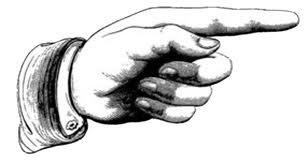
\includegraphics[width=3.5in]{Figure_1}
\caption{An overview of pointing with help of hand.}
\end{figure}

Pointing in a computer is done with various devices like mouse, joystick, trackball, touch-pad. In our project, we develop an application that enables pointing by fingers using a device called as Leap Motion Controller.

Leap Motion Controller is unique from other pointing device in a sense that, using this device as a pointing device, does not require a user to have a direct contact (or touch) with a computer screen. This device allows hand and finger as user inputs to interact with the computer. Figure 2 shows an overview of Leap Motion Controller. Figure 3 shows how a user can interact with the computer with help of Leap Motion Controller.

\begin{figure}[!h]
\centering
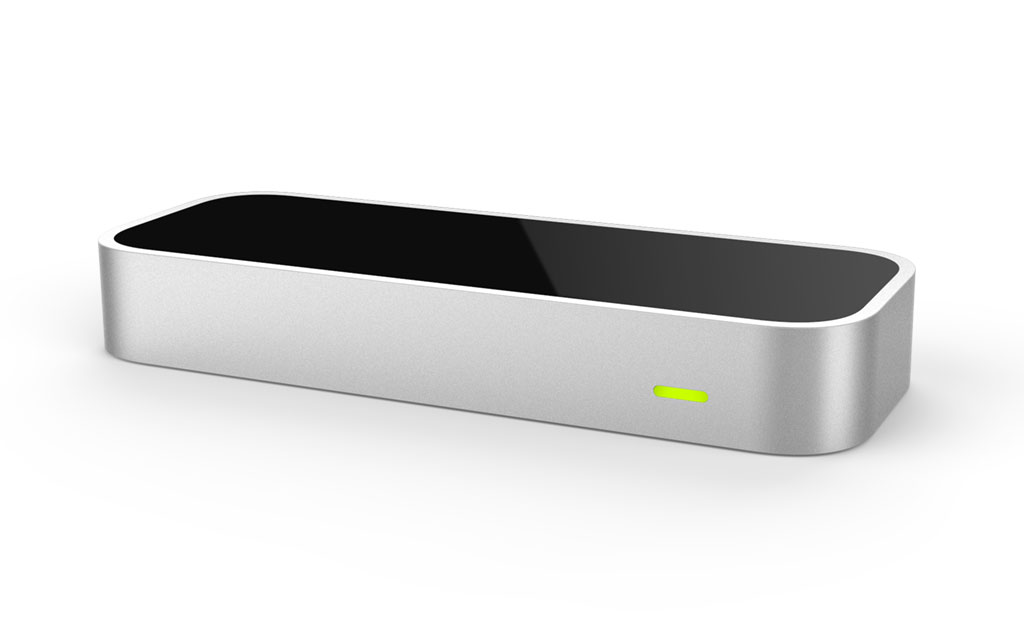
\includegraphics[width=3.5in]{Figure_2}
\caption{A Leap Motion Controller}
\end{figure}

\begin{figure}[!h]
\centering
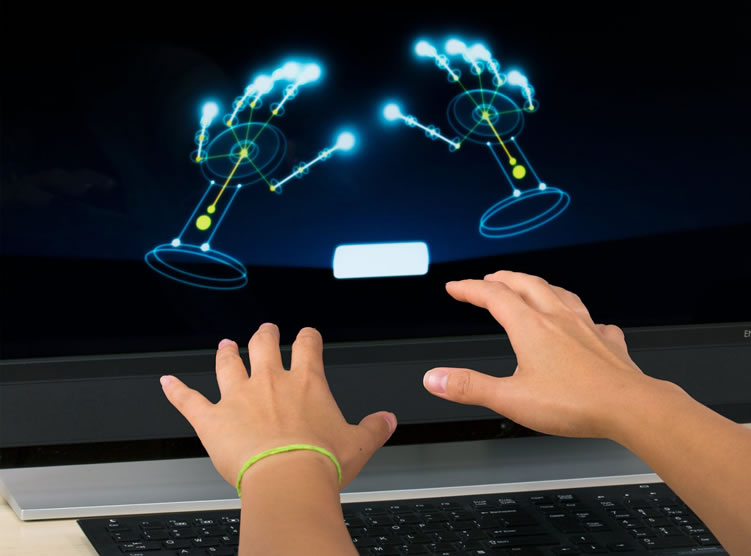
\includegraphics[width=3.5in]{Figure_3}
\caption{A user interacting with a computer using Leap Motion Controller.}
\end{figure}

Pointing are of two types: relative pointing and absolute pointing. Absolute pointing \cite{1} is direct pointing. Direct in this context means that there is a direct relation between the location of the pointing device and the cursor location. Few examples of direct pointing devices are touch screens, light pens and stylus boards. Relative pointing \cite{1} is indirect pointing. Indirect means that the user uses the pointing device to move the cursor from a starting point to an ending point, and there is no direct mapping between the device and the X, Y location on the screen. If the mouse reaches the edge of the mouse pad, the user can pick it up, put it back in the center of the mouse pad, and continue.   

\subsection{Application Description}

{\bf System requirements}:
\begin{itemize}
\item OS - Windows (version 7 or 8)
\item Pointing device - Leap Motion Controller
\item Framework - .NET 3.5 or above
\item Software - Leap Motion Software, Airspace, Unity 4 
\end{itemize}

{\bf Motive of the application}: The application developed in this project shows a comparison of ease of use of absolute pointing and relative pointing using Leap Motion Controller. In this application, a user performs the same task using two different pointing modes. 

{\bf User Interface description}: There are 4 filled balls of same size but different colors. There are 4 target circles of same size but different colors. The colors of the target circles are matched with the respective balls. The size of the target circles are bigger than the filled balls. When a user interacts with computer with help of a mouse, an arrow is shown as a cursor on the interface of the computer. In our project, when a user interacts with our application, a very small purple colored circle is shown as pointing circle (cursor). Whenever a user selects a filled ball, the color of the pointing circle changes. At the top, a timer shows the time to complete a single task.

{\bf Using the application}: The task that a user performs in two different pointing modes is to drag balls (filled with colors) to their respective target circles. The main menu of the application  provides a user (using this application) to choose between relative pointing mode and absolute pointing mode. For user feasibility, the application also provides an option for choosing between space bar grab mode and thumb grab mode. Space bar grab mode means, that the user can drag the filled balls towards the target circles with help of a space bar. Thumb grab mode means that the user can drag the filled balls with help of only thumb. This user feasibility has been introduced because Leap Motion Controller is quite new, hence users might find difficulty in dragging balls within the UI. We had tested our application with 3 users (all of them were new to Leap Motion Controller). All of them found difficulty in dragging the filled balls to their respective target circles, using only the thumb. Hence, we introduced the space bar mode, for user feasibility. After the space bar mode was introduced in the application, we repeated the same experiment with the same 3 users. This time users could use the application in much easier way. We record the time a user takes to complete a task using two pointing modes (absolute pointing and relative pointing).


\section{Background}
The idea of the project lies in showing the difference between relative pointing and absolute pointing. Relative pointing has got no direct relationship between the cursor of the pointing device and the position of the pointing device \cite{2}. On the other hand, absolute pointing there exists a direct relationship between the orientation of the pointing device and the cursor of the computer. These coordinates are gathered from with respect to fixed reference directions (for orientation) or fixed reference locations (for position) \cite{2}. Figure 4 shows the difference between relative pointing and absolute pointing. 

\begin{figure}[!h]
\centering
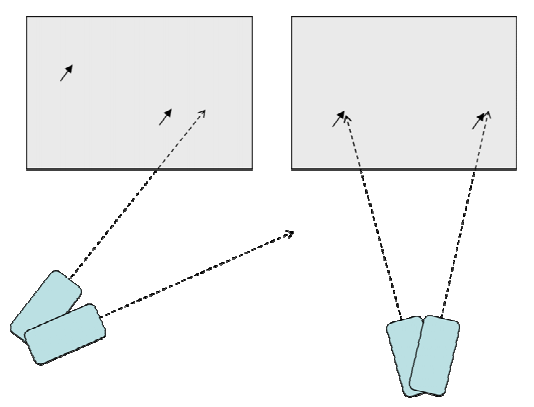
\includegraphics[width=3.5in]{Figure_4}
\caption{Illustrating the difference between relative (left) and absolute (right) pointing \cite{2}.}
\end{figure}

In our project, we demonstrate the difference between absolute pointing and relative pointing with the help of fingers. Vogel and Balakrishnan \cite{3} provide a design which demonstrates freehand pointing and clicking interaction with very large high resolution displays from a distance. The authors discuss about “Clicking and Clutching Without a Button”, which is the key point of our project. The authors have used hand gestures and postures for clicking. They argue that the click or clutch action should be designed in such manner that it minimizes hand movement side effects. This can be tedious due to the interconnectedness of tendons and ligaments in the hand. When a user selects or clicks a button, proper user feedback should be given so that the user is confirmed that the user has performed the task correctly. All of these user feed-backs are taken care of in our application.

\begin{figure}[!h]
\centering
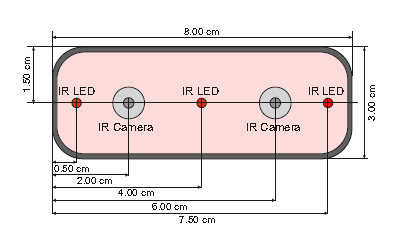
\includegraphics[width=3.5in]{Figure_5}
\caption{A schematic view of Leap Motion Controller \cite{4}.}
\end{figure}

Weichert et al. \cite{4} discuss about a new pointing device called Leap Motion Controller. This device has been used as the base of pointing device in our application. The Leap Motion Controller introduces a new methodology of interaction with the computers. It introduces a new gesture and position tracking system with sub-millimeter accuracy. The authors have shown the accuracy and robustness of the Leap Motion Controller. The controller is available to public and is currently been produced by Leap Motion \cite{5}. This controller calculates position in Cartesian space of predefined objects like finger tips, pen tip, etc. \cite{4}. These positions are in relation to the Leap Motion controller’s center point. The center point of the controller second infrared emitter. Figure 5 shows the schematic view of the Leap Motion Controller. The middle infrared emitter is the center point. It also consists of two infrared cameras. Figure 6 shows a top view of the Leap Motion Controller. The figure shows the position of the cameras in real life.

\section{Design}
This application allows a user to drag the circles to their respective target circles using two pointing modes (absolute pointing and relative pointing). The time to accomplish the task using both the pointing modes are being recorded. This application can act as a tool to compare between the two pointing modes to see if there are any identifiable differences in how effective each mode is compared to the other using Leap Motion Controller. 

The main concepts of the design of this application is modular design. The key design concepts are:

\begin{itemize}
  \item Separate scripts interacting with each other.
  \item Separation of UI from behaviour implementation.
\end{itemize}

\begin{figure}[!h]
\centering
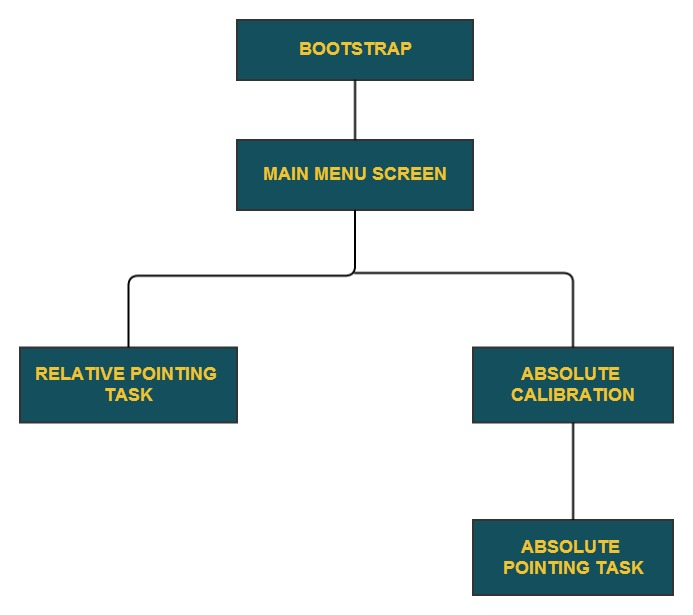
\includegraphics[width=4.5in]{Figure_6}
\caption{A higher level architecture of the application of this project.}
\end{figure}

The scripts responsible for user interface are:

\begin{itemize}
    \item Pointer.cs
    \item Circles.cs
    \item TaskTimer.cs
    \item KeyboardInput.cs
    \item LeapAsMouse.cs
    \item TitleGUI.cs
\end{itemize}

The scripts responsible for implementing the absolute and relative pointing concepts are:

\begin{itemize}
    \item LeapPointing.cs
    \item AppData.cs
    \item AbsoluteCalibration.cs

\end{itemize}

Figure 6 shows an overview of the higher level architecture of the application. The figure shows the main Unity scenes of the application.

The Bootstrap scene consists the following scripts:

\begin{itemize}
    \item AppData.cs
    \item KeyboardInput.cs
    \item LeapPointing.cs
\end{itemize}

KeyboardInput.cs script captures the keyboard input and updates global AppData. It uses the AppData to communicate with other scripts. The LeapPointing.cs script contains the code for both absolute pointing mode and relative pointing mode. This script updates the AppData.cs script with coordinates to communicate with other modules depending on the pointing mode selected in AppData. The AppData.cs script stores all the data that is used across multiple scenes. Figure 7 shows the functionality of the bootstrap scene.

\begin{figure}[!h]
\centering
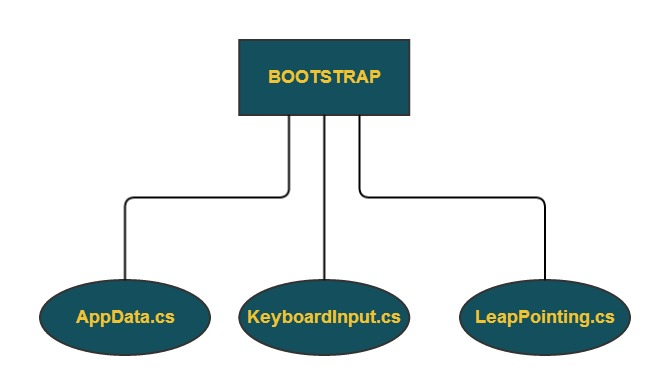
\includegraphics[width=4.5in]{Figure_7}
\caption{A higher level architecture of the application of this project.}
\end{figure}


The Bootstarp.cs script calls the main menu scene. It is to load the persistent DataObject to avoid duplication. The main menu scene consists of TitleGUI.cs script. It consist the user interface of the main menu. Figure 9 shows an overview of the interface of the main menu. This allows the user to choose between the two types of pointing modes. After choosing the required pointing mode, the user moves to the main application task area where the user performs the task of dragging circles.

\begin{figure}[!h]
\centering
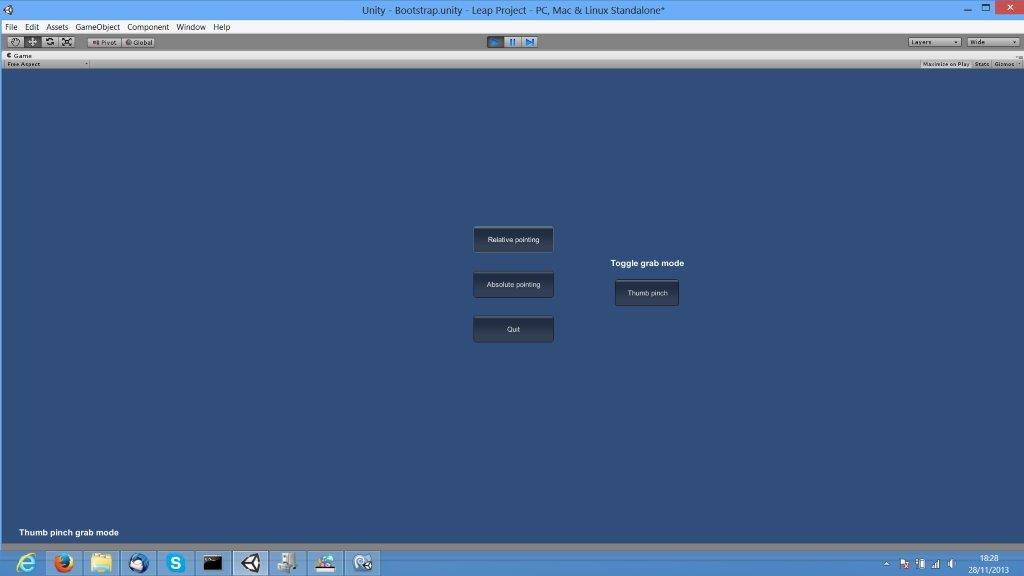
\includegraphics[width=7.0in]{Figure_8}
\caption{A screenshot of the main menu of the application.}
\end{figure}

The relative pointing task scene consists of the following scripts:

\begin{itemize}
    \item Pointer.cs
    \item Circles.cs
    \item TaskTimer.cs
\end{itemize}

Pointer.cs script draws purple colored pointer (which acts as cursor) to the screen coordinates. It updates the coordinates from the AppData.cs script. The Circles.cs script draws 4 circles and 4 target circles on the screen. It also records state of the circles - grabbed or not grabbed. If the user successfully grabs or selects a ball, then it changes the color of the circles. It also redraws the circles if the user cannot successfully drag the ball inside the target circles. The application also changes color when the center of the ball and the target circle matches providing a user feedback. The TaskTimer.cs script displays the time taken for a user to complete the full task of drag and drop of circles to the target circles. It starts recording the time when a user first selects a ball for dragging and ends when the user successfully drops the last ball to the target circle. Figure 10 shows internal flow diagram of relative pointing task scene. 

\begin{figure}[!h]
    \centering
    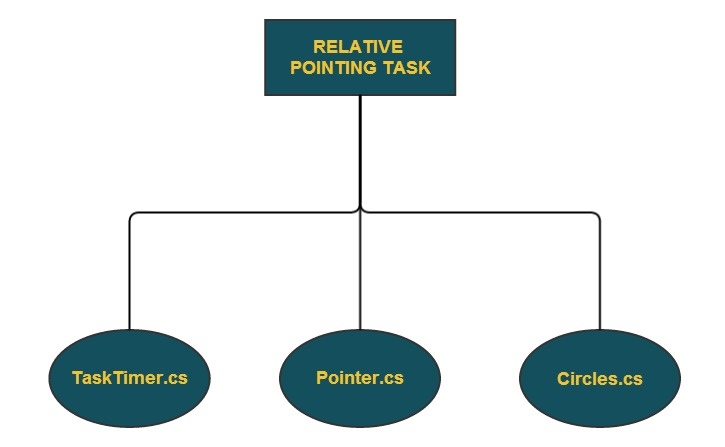
\includegraphics[width=4.5in]{Figure_9}
    \caption{Internal flow diagram of relative pointing task scene.}
\end{figure}
 

The AbsoluteCalibration.cs is the most important script for absolute pointing mode. The absoloute pointing mode uses this scaling ratios in its algorithm. The calibration script calculates the scaling ratios to create a relationship between leap position and screen dimensions. For scaling, it calculates the following data points:

\begin{itemize}
    \item 3 top left of screen
    \item 3 bottom right of the screen

\end{itemize}


The relativabsolute pointing task scene consists of the following scripts:

\begin{itemize}
    \item Pointer.cs
    \item Circles.cs
    \item TaskTimer.cs
    
\end{itemize}

The functionalities of each of the scripts have been explained above.

\section{Development}

The most significant elements of the application are the approaches taken for the relative and absolute pointing algorithms. Here a brief explanation of the relevant code contained in the LeapPointing script is provided.

\subsection{Relative pointing algorithm}
A zone is defined for the leap motion based on predefined values for width and height above table top. This 'zone' is effectively the space a user will be moving their finger around in above the Leap device. The height of the leap zone is then dynamically calculated based on the dimensions of the Unity window resulting in the Leap zone having the same ratio as the Unity screen.(figure 11)

\begin{figure}[!h]
    \centering
    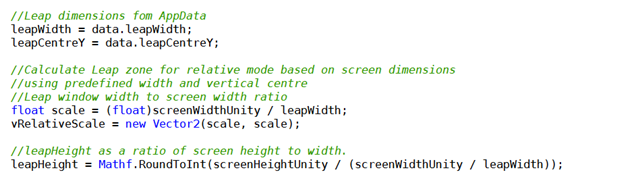
\includegraphics[width=7.0in]{Figure_10}
    \caption{Calculation of Leap zone dimensions.}
\end{figure}

The relative pointing algorithm takes raw data from the Leap in the form of the pre-stabilised position of the frontmost finger. The Leap coordinates (with X axis centred above the Leap device and Y zero located down at the device) are transformed to conform to Unity coordinates (0,0 top left) and adjusted to the dimensions of the previously defined Leap zone (figure 12).

\begin{figure}[!h]
    \centering
    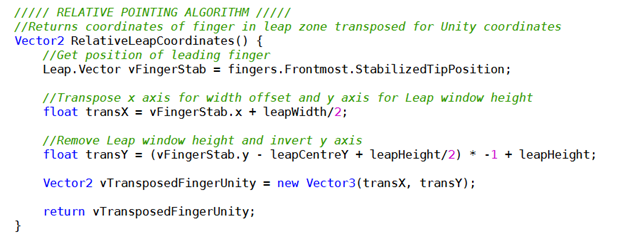
\includegraphics[width=7.0in]{Figure_11}
    \caption{Relative pointing algorithm.}
\end{figure}
 
The StabilizedTipPosition method offered by the Leap has very effective context-sensitive filtering and stabilisation, so no further smoothing is required.

Finally, when the application is in the RelativePointing mode (the relative pointing task screen as shown in Figure 14) the RelativePoint method (figure 13) gets the Unity adjusted coordinates from the  relative pointing algorithm and scales them to the screen dimensions using the Leap zone to screen size scaling value calculated in figure 11.

\begin{figure}[!h]
    \centering
    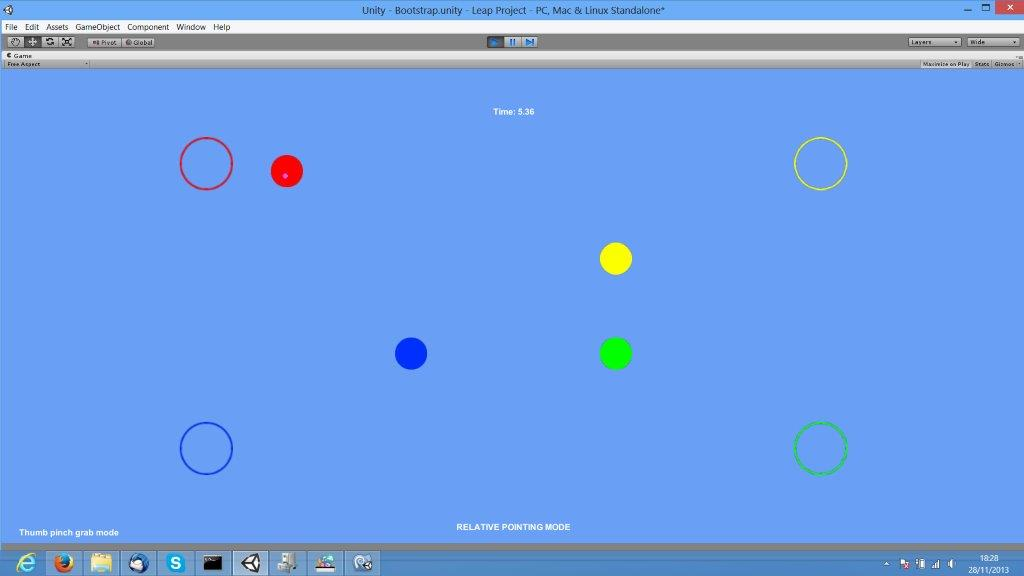
\includegraphics[width=7.0in]{Figure_13}
    \caption{RelativePoint method scaling results from relative pointing algorithm to screen size.}
\end{figure}

Figure 13 – RelativePoint method scaling results from relative pointing algorithm to screen size.
\begin{figure}[!h]
    \centering
    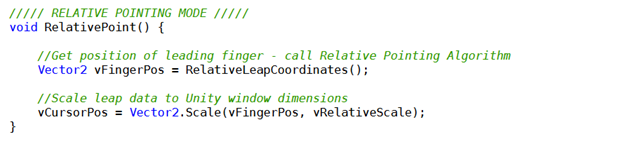
\includegraphics[width=7.0in]{Figure_12}
    \caption{A screenshot of relative pointing task scene of the application.}
\end{figure}


\subsection{Absolute Pointing}
The absolute algorithm (figure 15) makes use of a Leap feature where the angle of a finger is used to project a line onto a virtual screen which returns a coordinate where the projected line intersects with the virtual screen.
 
Initially the closest finger to the screen is defined. Then a virtual screen that that fingers projected line is intersecting with is identified, and the intersection coordinate is captured in vLeapIntersect.
 
After converting the Leap vector to a Vector2, the coordinates are scaled up from their normalised form to create a virtual screen with coordinates transposed to the Unity system.
 
To create the relationship between the virtual screen and the real screen, reference points (of top left and bottom right), which were defined during calibration, are used. The virtual screen coordinates are scaled to real window coordinates based on the ratio between virtual screen dimensions and the reference points (defining the real screen dimensions).
 
Finally smoothing is applied. This is required as the sensitivity of the Leap device means the pointer jumps around the screen due to natural tremors in the pointing finger.

\begin{figure}[!h]
    \centering
    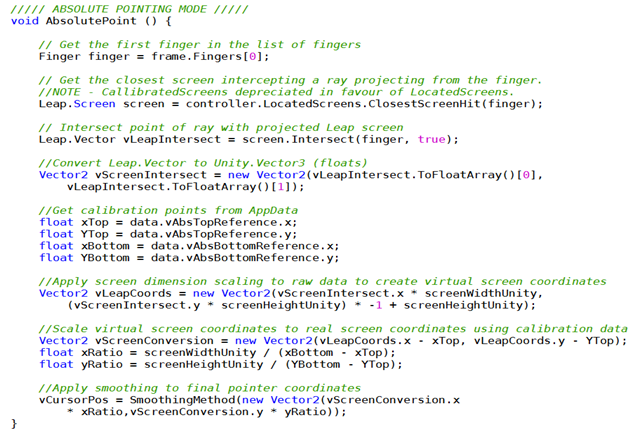
\includegraphics[width=7.0in]{Figure_14}
    \caption{A screenshot of relative pointing task scene of the application.}
\end{figure}

The smoothing algorithm (figure 16) employs a Savitzky-Golay algorithm. It applies
weighting coefficients to the last 9 frame coordinates giving prominence to the coordinates in the middle of the data set. This effectively fits the data into a polynomial which reduces the impact of noisy coordinates and produces a cosmetic smoothing effect for the pointer on screen.

\begin{figure}[!h]
    \centering
    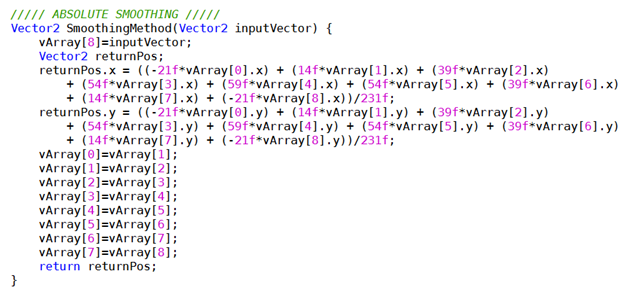
\includegraphics[width=7.0in]{Figure_15}
    \caption{Absolute pointing algorithm.}
\end{figure}

\section{Discussion}
The application developed in this project shows the comparison of absolute pointing and relative pointing with help of Leap motion controller. The very first challenge we faced was to narrow down to the programming language to be used for developing applications which use Leap Motion. As Leap Motion is still in its infancy, the documentation is not easy to follow, although its getting better. The next challenge was getting desired usability for users to be able to complete the tasks.  The last challenge in absolute pointing mode was pointer jitter problems. There were issues with pointer stability due to the Leap Motions high sensitivity and humans natural hand tremors. Hence to overcome this problem smoothing algorithm was used. Regarding the development of the application, the challenge was, according to the documentation of Lead SDK, it could be used as a plug-in in a Unity application using Pro version of Unity. Anyways using some tweaks, we got to interact with a sample unity application using leap motion with a free version too. Also, the main requirement of the application development was Leap Motion Controller. Given a team size of 5 members, only one controller was available. If one more controller was available then the development process would have been easier and convenient. The availability of the Leap Motion controller was a problem. Also, the Leap Motion controller had stopped working twice. It might be a bug of the Controller. After un-installing and reinstalling the leap software, the device started working once again.



\section{Conclusion}
This project shows an application that compares the ease of use between absolute pointing and relative pointing using Leap Motion Controller. The finger is considered as the mode of pointing. This project integrates Leap Motion controller with Unity. It captures the quantifiable data in order to assess the effectiveness of different pointing techniques using a Leap Motion Controller. 


\bibliography{if.bib}
\bibliographystyle{plain}

\end{document}
